\section{Preliminary Experiments on ColourBomb}

This section reports only completed ColourBomb runs from \texttt{runs/cb}. The analysis is fully data-driven from stored \texttt{baseline\_metrics.csv} files and seed aggregation artifacts generated by \texttt{paper/scripts/build\_cb\_figures.py}.

\subsection{Alpha Sensitivity: Invariant Safety (\texttt{avoid\_bombs})}
Figure~\ref{fig:cb_alpha_avoid} shows the effect of logic weight $\alpha$ on invariant safety. The trend is non-monotonic: moderate values do not consistently improve over vanilla, while $\alpha=0.4$ gives the best safety among tested values.

\begin{figure}[t]
\centering

\includegraphics[width=\linewidth]{figures/colourbomb/cb_alpha_sweep_avoid_bombs.png}
\caption{ColourBomb, \texttt{avoid\_bombs}, greedy decoding. Mean and std over seeds $\{0,1,2\}$ across $\alpha \in \{0, 0.01, 0.05, 0.1, 0.2, 0.4\}$.}
\label{fig:cb_alpha_avoid}
\end{figure}

\begin{figure}[t]
\centering
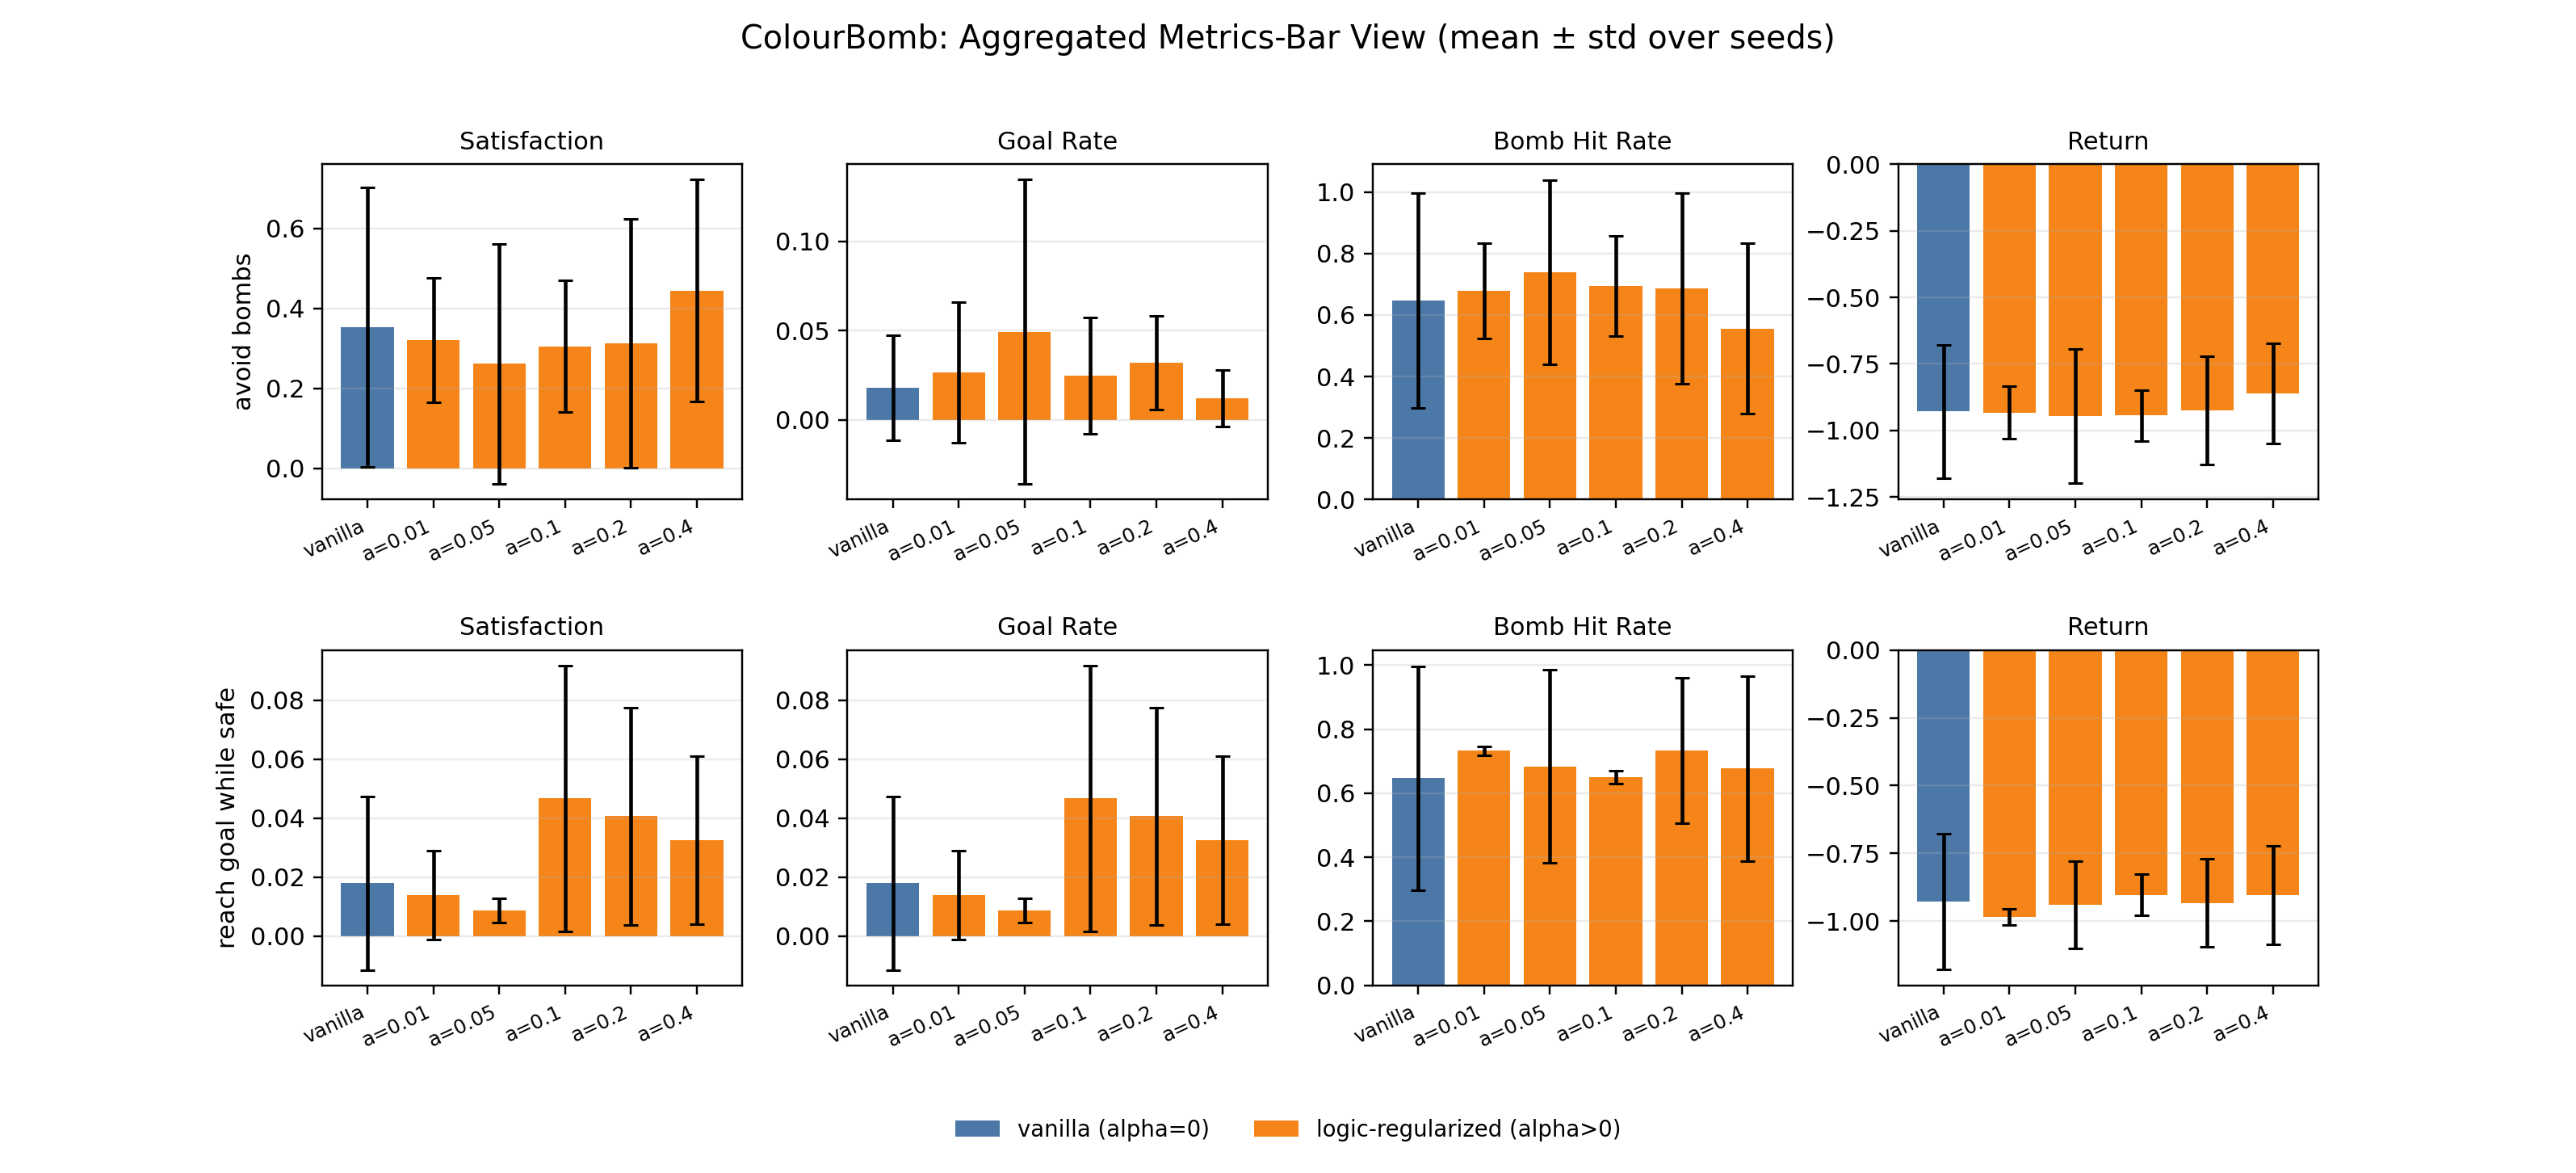
\includegraphics[width=\linewidth]{figures/colourbomb/cb_metrics_bar_example.png}
\caption{Improved metrics-bar style summary (aggregated over seeds) for both CB specs. This figure is the publication-style replacement for per-run \texttt{metrics\_bar} plots.}
\label{fig:cb_metrics_bar_example}
\end{figure}

\subsection{Alpha Sensitivity: Reach-While-Safe (\texttt{reach\_goal\_while\_safe})}
Figure~\ref{fig:cb_alpha_tradeoff} highlights the harder temporal objective. Satisfaction and goal rates are substantially lower than the invariant-only case. The best point in this sweep is around $\alpha=0.1$, but absolute performance remains limited, indicating a difficult goal-safety trade-off in the current CB setup.

\begin{figure}[t]
\centering
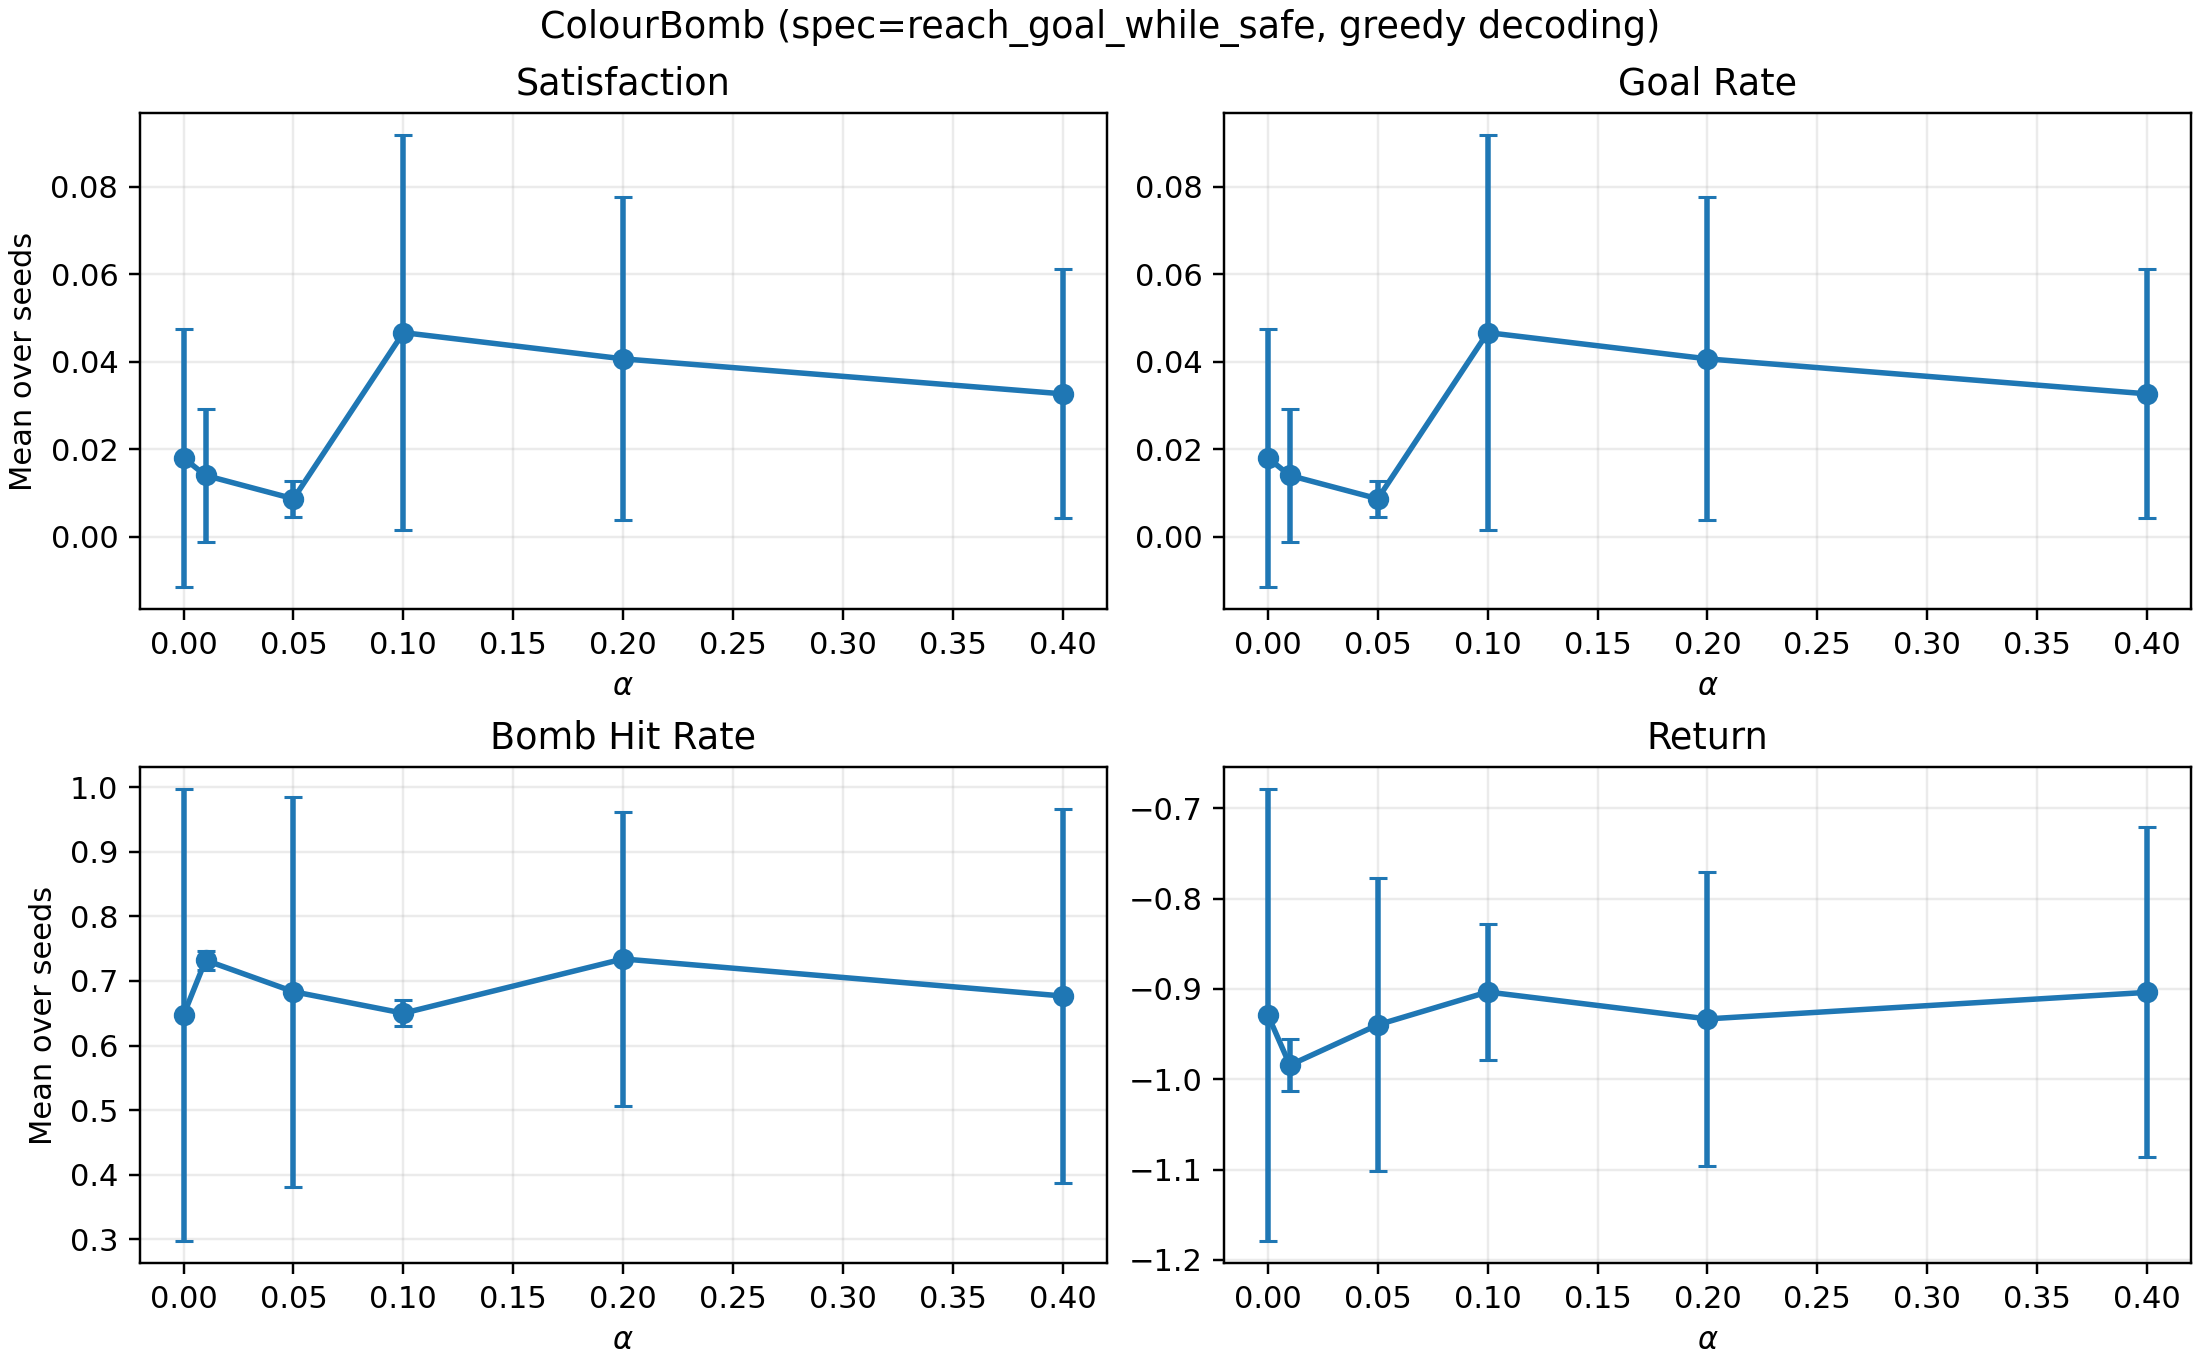
\includegraphics[width=\linewidth]{figures/colourbomb/cb_alpha_sweep_reach_goal_while_safe.png}
\caption{ColourBomb, \texttt{reach\_goal\_while\_safe}, greedy decoding. Mean and std over seeds $\{0,1,2\}$.}
\label{fig:cb_alpha_tradeoff}
\end{figure}

\subsection{Cross-Spec Comparison}
Figure~\ref{fig:cb_cross_spec} compares the best-satisfaction alpha per spec. The invariant objective can be improved mainly by reducing bomb hits, while the reach-while-safe objective remains constrained by low goal attainment.

\begin{figure}[t]
\centering
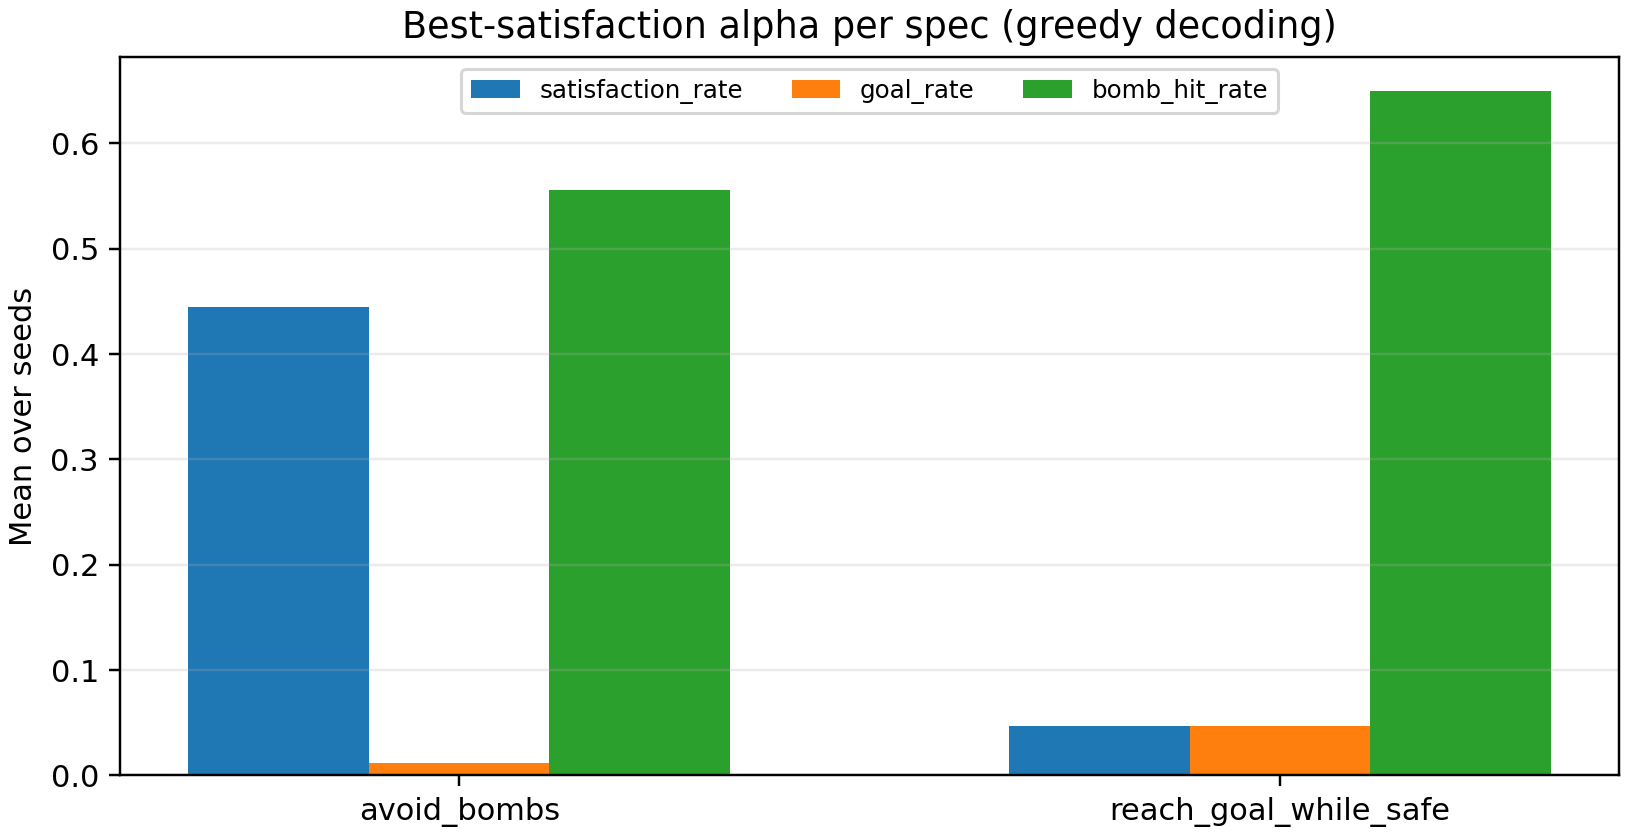
\includegraphics[width=0.9\linewidth]{figures/colourbomb/cb_spec_comparison_goal_vs_safety.png}
\caption{Best-satisfaction alpha per spec (greedy decoding), aggregated over three seeds.}
\label{fig:cb_cross_spec}
\end{figure}

\subsection{Key Quantitative Summary}
Table~\ref{tab:cb_key_results} reports representative operating points from the aggregated CB alpha table.

\begin{table}[t]
\caption{ColourBomb key results (means over seeds 0,1,2; greedy decoding).}
\label{tab:cb_key_results}
\centering
\small
\begin{tabular}{llcccc}
\toprule
Spec & Setting & Satisfaction & Goal & Bomb hit & Return \\
\midrule
\texttt{avoid\_bombs} & vanilla ($\alpha=0$) & 0.353 & 0.018 & 0.647 & -0.929 \\
\texttt{avoid\_bombs} & logic ($\alpha=0.4$) & \textbf{0.445} & 0.012 & \textbf{0.555} & \textbf{-0.862} \\
\texttt{avoid\_bombs} & logic ($\alpha=0.05$) & 0.261 & \textbf{0.049} & 0.739 & -0.946 \\
\midrule
\texttt{reach\_goal\_while\_safe} & vanilla ($\alpha=0$) & 0.018 & 0.018 & 0.647 & -0.929 \\
\texttt{reach\_goal\_while\_safe} & logic ($\alpha=0.1$) & \textbf{0.047} & \textbf{0.047} & 0.650 & \textbf{-0.903} \\
\bottomrule
\end{tabular}
\end{table}

\paragraph{Interpretation.}
The CB experiments support two practical conclusions.
\begin{itemize}
\item Logic regularization can improve safety-oriented metrics, but sensitivity to $\alpha$ is strong and not monotonic.
\item On the harder temporal spec (\texttt{reach\_goal\_while\_safe}), improvements are present but modest; increasing satisfaction currently correlates with only small gains in goal success.
\end{itemize}
